\section{方程问题}
\label{sec:hj-problem}

先把两类问题摆出来。一类问波前什么时候到达，未知函数不含时间；另一类问一个高度场随时间怎样变化，它的变化率由局部斜率决定。前者可以看成后者的特例，两者需要的数据却不一样。

\paragraph{到达时间}
从一维开始。在$x=0$处点火，火线以速度$c(x)>0$向右推进。经过一小段$[x,x+\mathrm{d}x]$需要的时间是$\mathrm{d}x/c(x)$，把这些时间加起来得到到达时间
\[
  T(x)=\int_0^x\frac{\mathrm{d}s}{c(s)},\qquad T'(x)=\frac{1}{c(x)}.
\]
速度越小，到达时间增长得越快，$T$的斜率就是“慢度”$1/c$。

取一组具体的速度：在$[0,1)$上$c=1$，在$[1,2)$上$c=0.4$，在$[2,3]$上$c=1.5$。逐段累加，得到
\[
  T(1)=1,\qquad T(2)=1+\frac{1}{0.4}=3.5,\qquad T(3)=3.5+\frac{1}{1.5}\approx4.17.
\]
图~\ref{fig:hj-arrival-1d}显示，$T$是折线，慢的中间一段最陡。

\begin{BookInlineFigure}
  \centering
  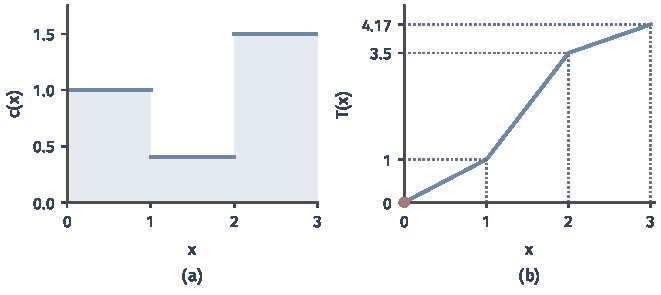
\includegraphics[width=112mm]{figures/06-differential-equations/02-partial-differential-equations/matplotlib/hj-arrival-1d/figure.pdf}
  \caption{一维到达时间。(a)分段常数的速度$c(x)$。(b)由$x=0$（红点）出发的到达时间$T(x)$，各段斜率是$1/c$。}
  \label{fig:hj-arrival-1d}
\end{BookInlineFigure}

到了高维，时刻$t$的波前是等值面$\{T=t\}$，已经被扫过的区域是$\{T\leq t\}$。设波前沿法向以速度$c(\bm{x})$推进。图~\ref{fig:hj-front-normal}中，点$\bm{x}$在$\mathrm{d}t$后沿法向$\bm{n}$到达$\bm{x}+c\,\mathrm{d}t\,\bm{n}$，那里的到达时间恰好多了$\mathrm{d}t$，所以
\[
  \langle\nabla T,\ c\,\bm{n}\rangle\,\mathrm{d}t=\mathrm{d}t.
\]
法向是$T$增长的方向，$\bm{n}=\nabla T/\lVert\nabla T\rVert_2$。代入后得到$c\,\lVert\nabla T\rVert_2=1$。

\begin{BookInlineFigure}
  \centering
  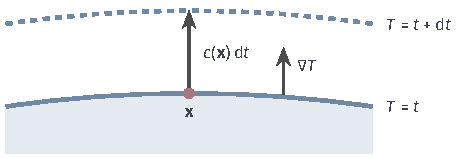
\includegraphics[width=78.3mm]{figures/06-differential-equations/02-partial-differential-equations/tikz/hj-front-normal/figure.pdf}
  \caption{波前的法向推进。实线是时刻$t$的波前，虚线是$t+\mathrm{d}t$的波前，浅蓝是已扫过的区域。两条等值线的法向距离是$c(\bm{x})\,\mathrm{d}t$，所以$\nabla T$的长度是$1/c$。}
  \label{fig:hj-front-normal}
\end{BookInlineFigure}

这个局部关系连同“从哪里开始、何时开始”的数据，构成到达时间问题。

\begin{definition}[程函方程]
\label{def:hj-eikonal}
设$\Omega\subset\mathbb{R}^{d}$是开集，$c:\Omega\to(0,\infty)$连续，$\Gamma\subset\overline{\Omega}$是闭集，$g:\Gamma\to\mathbb{R}$是给定的起始时刻。称
\begin{equation}
  c(\bm{x})\,\lVert\nabla T(\bm{x})\rVert_2=1\quad(\bm{x}\in\Omega\setminus\Gamma),\qquad
  T=g\quad\text{在}\ \Gamma\ \text{上}
  \label{eq:hj-eikonal}
\end{equation}
为\term{程函方程}（eikonal equation）的边值问题，$T$称为\term{到达时间}（arrival time），它的等值面$\{T=t\}$称为时刻$t$的\term{波前}（wavefront）。
\end{definition}

方程里没有时间，时间是未知函数的取值。一维时方程写作$\lvert T'\rvert=1/c$，比前面的$T'=1/c$少了方向信息：向左走还是向右走，方程本身不管。第~\ref{chap:pde-problems}章已经见过这种缺失带来的后果，$\lvert u'\rvert=1$、$u(\pm1)=0$没有$C^1$解，却有无穷多条几乎处处满足方程的锯齿线。

\paragraph{初值演化}
到达时间也可以放进一个随时间变化的场里。令$u(\bm{x},t)=T(\bm{x})-t$，则时刻$t$的波前就是$u(\cdot,t)$的零等值面。这时$\partial_tu=-1$，$\nabla u=\nabla T$，所以程函方程变成
\[
  \partial_tu+c(\bm{x})\,\lVert\nabla u\rVert_2=0.
\]
图~\ref{fig:hj-level-set}对$T(x)=\lvert x\rvert$画出这件事：函数图像整体下降，零点（红）就是向两侧跑的波前。

\begin{BookInlineFigure}
  \centering
  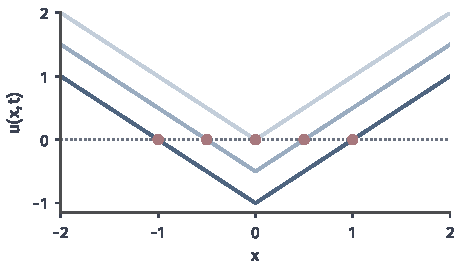
\includegraphics[width=78mm]{figures/06-differential-equations/02-partial-differential-equations/matplotlib/hj-level-set/figure.pdf}
  \caption{把波前写成零等值面。蓝色由浅到深是$u(x,t)=\lvert x\rvert-t$在$t=0,0.5,1$的图像，红点是零点$x=\pm t$，它们以速度$1$向两侧运动。}
  \label{fig:hj-level-set}
\end{BookInlineFigure}

把$c\lVert\bm{p}\rVert_2$换成一般的函数，就得到本章的第二类问题。

\begin{definition}[Hamilton--Jacobi初值问题]
\label{def:hj-ivp}
设$t_{\mathrm{f}}>0$，函数$H(t,\bm{x},\bm{p})$在$t\in[0,t_{\mathrm{f}}]$、$\bm{x},\bm{p}\in\mathbb{R}^{d}$上连续，$u_0$在$\mathbb{R}^{d}$上连续。称
\begin{equation}
  \partial_tu+H(t,\bm{x},\nabla u)=0\quad(\bm{x}\in\mathbb{R}^{d},\ 0<t<t_{\mathrm{f}}),\qquad
  u(\bm{x},0)=u_0(\bm{x})
  \label{eq:hj-ivp}
\end{equation}
为\term{Hamilton--Jacobi方程}（Hamilton--Jacobi equation）的初值问题，$H(t,\bm{x},\bm{p})$称为\term{Hamilton量}（Hamiltonian）。若$u$连续可微并逐点满足方程，就称$u$是经典解。
\end{definition}

本章的$u$只在$H$中通过梯度出现，$H$不依赖场值。比第~\ref{chap:transport-equations}章多出来的是：$H$对$\bm{p}$可以是非线性的。输运方程$\partial_tu+\langle\bm{v},\nabla u\rangle=0$正是$H=\langle\bm{v},\bm{p}\rangle$的线性情形。

\paragraph{Hamilton量的作用}
$H$回答的问题是：斜率为$\bm{p}$的地方，高度以多快的速度下降。这一点在平面解上能直接看出。对只依赖$\bm{p}$的$H$，令
\begin{equation}
  u(\bm{x},t)=\langle\bm{p},\bm{x}\rangle-tH(\bm{p}).
  \label{eq:hj-plane-solution}
\end{equation}
此时$\nabla u=\bm{p}$，$\partial_tu=-H(\bm{p})$，方程逐点成立。斜率不变，整个平面以速率$H(\bm{p})$下降。

图~\ref{fig:hj-plane-slopes}取$H(p)=p^2/2$。斜率$p=0,1,2$的三条直线在$t=1$时分别下降$0$、$0.5$和$2$。下降量对斜率是二次的。把两个斜率为$1$的解相加，得到的直线斜率为$2$，下降量却只有$1$，而斜率为$2$的解应当下降$2$，所以解不能叠加。

\begin{BookInlineFigure}
  \centering
  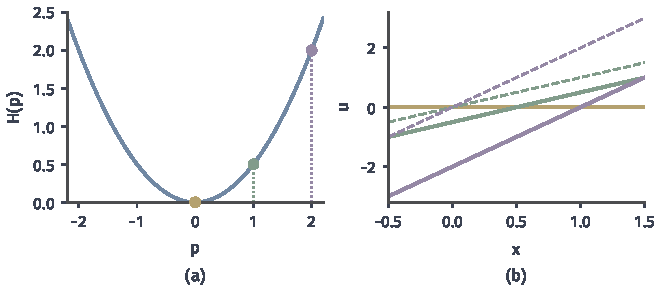
\includegraphics[width=112mm]{figures/06-differential-equations/02-partial-differential-equations/matplotlib/hj-plane-slopes/figure.pdf}
  \caption{Hamilton量决定下降速率。(a)$H(p)=p^2/2$，三个点对应$p=0,1,2$（黄、绿、紫）。(b)对应的平面解，虚线是$t=0$，实线是$t=1$，下降量分别是$0$、$0.5$、$2$。}
  \label{fig:hj-plane-slopes}
\end{BookInlineFigure}

一维时方程和第~\ref{chap:scalar-conservation-laws}章的守恒律有直接的关系。设$H=H(p)$，$u$足够光滑，对$\partial_tu+H(\partial_xu)=0$再求一次$x$偏导，$v=\partial_xu$满足
\[
  \partial_tv+\partial_xH(v)=0.
\]
所以一维的Hamilton--Jacobi方程是通量为$H$的标量守恒律的“原函数”，$u$的折角对应$v$的间断。这个对应后面会反复用到，但它只在一维成立；高维时梯度是向量，不满足标量守恒律。

\paragraph{两类问题需要的数据}
表~\ref{tab:hj-two-problems}把两类问题放在一起。两者都是对梯度的非线性方程，数据的位置和要求不同。

\begin{BookInlineTable}
  \centering
  \begin{tabular}{lll}
    \toprule
    & 到达时间问题 & 初值演化问题\\
    \midrule
    未知量 & $T(\bm{x})$，时间是取值 & $u(\bm{x},t)$\\
    梯度的含义 & 慢度向量，长度$1/c$ & 局部斜率\\
    方程的作用 & 限制梯度的长度 & 由斜率给出下降速率\\
    所需数据 & 源集合$\Gamma$上的起始时刻 & $t=0$时整个$\mathbb{R}^{d}$上的$u_0$\\
    数据的限制 & 起始时刻不能相互矛盾 & 增长和正则性\\
    \bottomrule
  \end{tabular}
  \caption{到达时间问题与初值演化问题的对比。}
  \label{tab:hj-two-problems}
\end{BookInlineTable}

初值问题只需要在$t=0$给一个函数，方程对时间是一阶的，不需要初始速度，全空间上也没有侧边界。到达时间问题的数据要彼此相容。在区间$(0,1)$上取$c=1$，两端都是源，起始时刻为$g(0)=0$和$g(1)=2$。从左端出发的波前在时刻$1$就到达了右端，而右端规定的起始时刻是$2$，这个规定不会起作用。一般的要求是，$\lvert g(\bm{x})-g(\bm{y})\rvert$不超过两点之间的传播时间；这个限制在第~\ref{sec:hj-comparison}节还要用到。
